\documentclass[twoside]{book}

% Packages required by doxygen
\usepackage{calc}
\usepackage{doxygen}
\usepackage{graphicx}
\usepackage[utf8]{inputenc}
\usepackage{makeidx}
\usepackage{multicol}
\usepackage{multirow}
\usepackage{textcomp}
\usepackage[table]{xcolor}

% Font selection
\usepackage[T1]{fontenc}
\usepackage{mathptmx}
\usepackage[scaled=.90]{helvet}
\usepackage{courier}
\usepackage{amssymb}
\usepackage{sectsty}
\renewcommand{\familydefault}{\sfdefault}
\allsectionsfont{%
  \fontseries{bc}\selectfont%
  \color{darkgray}%
}
\renewcommand{\DoxyLabelFont}{%
  \fontseries{bc}\selectfont%
  \color{darkgray}%
}

% Page & text layout
\usepackage{geometry}
\geometry{%
  a4paper,%
  top=2.5cm,%
  bottom=2.5cm,%
  left=2.5cm,%
  right=2.5cm%
}
\tolerance=750
\hfuzz=15pt
\hbadness=750
\setlength{\emergencystretch}{15pt}
\setlength{\parindent}{0cm}
\setlength{\parskip}{0.2cm}
\makeatletter
\renewcommand{\paragraph}{%
  \@startsection{paragraph}{4}{0ex}{-1.0ex}{1.0ex}{%
    \normalfont\normalsize\bfseries\SS@parafont%
  }%
}
\renewcommand{\subparagraph}{%
  \@startsection{subparagraph}{5}{0ex}{-1.0ex}{1.0ex}{%
    \normalfont\normalsize\bfseries\SS@subparafont%
  }%
}
\makeatother

% Headers & footers
\usepackage{fancyhdr}
\pagestyle{fancyplain}
\fancyhead[LE]{\fancyplain{}{\bfseries\thepage}}
\fancyhead[CE]{\fancyplain{}{}}
\fancyhead[RE]{\fancyplain{}{\bfseries\leftmark}}
\fancyhead[LO]{\fancyplain{}{\bfseries\rightmark}}
\fancyhead[CO]{\fancyplain{}{}}
\fancyhead[RO]{\fancyplain{}{\bfseries\thepage}}
\fancyfoot[LE]{\fancyplain{}{}}
\fancyfoot[CE]{\fancyplain{}{}}
\fancyfoot[RE]{\fancyplain{}{\bfseries\scriptsize Generated on Wed Jun 15 2016 11\-:51\-:53 for D\-S\-P\-I by Doxygen }}
\fancyfoot[LO]{\fancyplain{}{\bfseries\scriptsize Generated on Wed Jun 15 2016 11\-:51\-:53 for D\-S\-P\-I by Doxygen }}
\fancyfoot[CO]{\fancyplain{}{}}
\fancyfoot[RO]{\fancyplain{}{}}
\renewcommand{\footrulewidth}{0.4pt}
\renewcommand{\chaptermark}[1]{%
  \markboth{#1}{}%
}
\renewcommand{\sectionmark}[1]{%
  \markright{\thesection\ #1}%
}

% Indices & bibliography
\usepackage{natbib}
\usepackage[titles]{tocloft}
\setcounter{tocdepth}{3}
\setcounter{secnumdepth}{5}
\makeindex

% Hyperlinks (required, but should be loaded last)
\usepackage{ifpdf}
\ifpdf
  \usepackage[pdftex,pagebackref=true]{hyperref}
\else
  \usepackage[ps2pdf,pagebackref=true]{hyperref}
\fi
\hypersetup{%
  colorlinks=true,%
  linkcolor=blue,%
  citecolor=blue,%
  unicode%
}

% Custom commands
\newcommand{\clearemptydoublepage}{%
  \newpage{\pagestyle{empty}\cleardoublepage}%
}


%===== C O N T E N T S =====

\begin{document}

% Titlepage & ToC
\hypersetup{pageanchor=false}
\pagenumbering{roman}
\begin{titlepage}
\vspace*{7cm}
\begin{center}%
{\Large D\-S\-P\-I \\[1ex]\large 1 }\\
\vspace*{1cm}
{\large Generated by Doxygen 1.8.6}\\
\vspace*{0.5cm}
{\small Wed Jun 15 2016 11:51:53}\\
\end{center}
\end{titlepage}
\clearemptydoublepage
\tableofcontents
\clearemptydoublepage
\pagenumbering{arabic}
\hypersetup{pageanchor=true}

%--- Begin generated contents ---
\chapter{Hierarchical Index}
\section{Class Hierarchy}
This inheritance list is sorted roughly, but not completely, alphabetically\-:\begin{DoxyCompactList}
\item \contentsline{section}{config}{\pageref{d5/d86/structconfig}}{}
\item \contentsline{section}{Config\-File}{\pageref{dc/d25/classConfigFile}}{}
\item \contentsline{section}{file\-Properties}{\pageref{d0/d01/structfileProperties}}{}
\item \contentsline{section}{Menu\-Component}{\pageref{d2/dfd/classMenuComponent}}{}
\begin{DoxyCompactList}
\item \contentsline{section}{Menu\-Composition}{\pageref{d3/d20/classMenuComposition}}{}
\item \contentsline{section}{Menu\-Primitive}{\pageref{dd/db3/classMenuPrimitive}}{}
\end{DoxyCompactList}
\item \contentsline{section}{my\-Daemon}{\pageref{da/d80/classmyDaemon}}{}
\item \contentsline{section}{server\-Params}{\pageref{dc/da3/structserverParams}}{}
\item \contentsline{section}{spi}{\pageref{d0/d2e/classspi}}{}
\item \contentsline{section}{spi\-Params}{\pageref{d9/d23/structspiParams}}{}
\item \contentsline{section}{spi\-Params\-Str}{\pageref{d5/ddd/structspiParamsStr}}{}
\item \contentsline{section}{time\-Date}{\pageref{df/da2/structtimeDate}}{}
\end{DoxyCompactList}

\chapter{Class Index}
\section{Class List}
Here are the classes, structs, unions and interfaces with brief descriptions\-:\begin{DoxyCompactList}
\item\contentsline{section}{\hyperlink{structconfig}{config} }{\pageref{d5/d86/structconfig}}{}
\item\contentsline{section}{\hyperlink{classConfigFile}{Config\-File} }{\pageref{dc/d25/classConfigFile}}{}
\item\contentsline{section}{\hyperlink{structfileProperties}{file\-Properties} }{\pageref{d0/d01/structfileProperties}}{}
\item\contentsline{section}{\hyperlink{classMenuComponent}{Menu\-Component} }{\pageref{d2/dfd/classMenuComponent}}{}
\item\contentsline{section}{\hyperlink{classMenuComposition}{Menu\-Composition} }{\pageref{d3/d20/classMenuComposition}}{}
\item\contentsline{section}{\hyperlink{classMenuPrimitive}{Menu\-Primitive} }{\pageref{dd/db3/classMenuPrimitive}}{}
\item\contentsline{section}{\hyperlink{classmyDaemon}{my\-Daemon} }{\pageref{da/d80/classmyDaemon}}{}
\item\contentsline{section}{\hyperlink{structserverParams}{server\-Params} }{\pageref{dc/da3/structserverParams}}{}
\item\contentsline{section}{\hyperlink{classspi}{spi} }{\pageref{d0/d2e/classspi}}{}
\item\contentsline{section}{\hyperlink{structspiParams}{spi\-Params} }{\pageref{d9/d23/structspiParams}}{}
\item\contentsline{section}{\hyperlink{structspiParamsStr}{spi\-Params\-Str} }{\pageref{d5/ddd/structspiParamsStr}}{}
\item\contentsline{section}{\hyperlink{structtimeDate}{time\-Date} }{\pageref{df/da2/structtimeDate}}{}
\end{DoxyCompactList}

\chapter{Class Documentation}
\hypertarget{structconfig}{\section{config Struct Reference}
\label{structconfig}\index{config@{config}}
}
\subsection*{Public Attributes}
\begin{DoxyCompactItemize}
\item 
\hypertarget{structconfig_affd1e4fdeeb5bd09b7f037fe642932a9}{const std\-::string {\bfseries \-\_\-daemon\-Dir} = \char`\"{}/var/run\char`\"{}}\label{structconfig_affd1e4fdeeb5bd09b7f037fe642932a9}

\item 
\hypertarget{structconfig_ab4f00bce3683d1c2464380b3631ef2f2}{const std\-::string {\bfseries \-\_\-daemon\-Pid\-File} = \char`\"{}/var/run/dspi.\-pid\char`\"{}}\label{structconfig_ab4f00bce3683d1c2464380b3631ef2f2}

\item 
\hypertarget{structconfig_ae0091570b7bee3d1b418f3c0f9ae446e}{std\-::string {\bfseries \-\_\-app\-Name}}\label{structconfig_ae0091570b7bee3d1b418f3c0f9ae446e}

\item 
\hypertarget{structconfig_a720319d92313892a3cb3094f7dcf4730}{\hyperlink{structspiParamsStr}{spi\-Params\-Str} {\bfseries \-\_\-spi\-Params}}\label{structconfig_a720319d92313892a3cb3094f7dcf4730}

\item 
\hypertarget{structconfig_aa8294046e3a51d625db081163c63b438}{\hyperlink{structserverParams}{server\-Params} {\bfseries \-\_\-server\-Params}}\label{structconfig_aa8294046e3a51d625db081163c63b438}

\end{DoxyCompactItemize}


The documentation for this struct was generated from the following file\-:\begin{DoxyCompactItemize}
\item 
Config\-File.\-h\end{DoxyCompactItemize}

\hypertarget{classConfigFile}{\section{Config\-File Class Reference}
\label{classConfigFile}\index{Config\-File@{Config\-File}}
}
\subsection*{Public Member Functions}
\begin{DoxyCompactItemize}
\item 
\hyperlink{classConfigFile_a9ce259defdfaabeedb2455849ca6bd1e}{Config\-File} ()
\item 
\hyperlink{classConfigFile_ab5c5ee702366f5f4c8833bfe58dfe306}{Config\-File} (const \hyperlink{classConfigFile}{Config\-File} \&orig)
\item 
virtual \hyperlink{classConfigFile_ae73765f7f0320bb6422da1cebe866f31}{$\sim$\-Config\-File} ()
\item 
void \hyperlink{classConfigFile_a525b771d6c5df54fe40c0d4aedeeaf02}{Read\-Config\-Params} ()
\item 
\hypertarget{classConfigFile_aa12085de76fa6eabef7d0d23938a4279}{\hyperlink{structconfig}{config} $\ast$ {\bfseries get\-Config\-Params} ()}\label{classConfigFile_aa12085de76fa6eabef7d0d23938a4279}

\end{DoxyCompactItemize}


\subsection{Constructor \& Destructor Documentation}
\hypertarget{classConfigFile_a9ce259defdfaabeedb2455849ca6bd1e}{\index{Config\-File@{Config\-File}!Config\-File@{Config\-File}}
\index{Config\-File@{Config\-File}!ConfigFile@{Config\-File}}
\subsubsection[{Config\-File}]{\setlength{\rightskip}{0pt plus 5cm}Config\-File\-::\-Config\-File (
\begin{DoxyParamCaption}
{}
\end{DoxyParamCaption}
)}}\label{classConfigFile_a9ce259defdfaabeedb2455849ca6bd1e}
Constructor \hypertarget{classConfigFile_ab5c5ee702366f5f4c8833bfe58dfe306}{\index{Config\-File@{Config\-File}!Config\-File@{Config\-File}}
\index{Config\-File@{Config\-File}!ConfigFile@{Config\-File}}
\subsubsection[{Config\-File}]{\setlength{\rightskip}{0pt plus 5cm}Config\-File\-::\-Config\-File (
\begin{DoxyParamCaption}
\item[{const {\bf Config\-File} \&}]{orig}
\end{DoxyParamCaption}
)}}\label{classConfigFile_ab5c5ee702366f5f4c8833bfe58dfe306}
Copy constructor 
\begin{DoxyParams}{Parameters}
{\em orig} & \\
\hline
\end{DoxyParams}
\hypertarget{classConfigFile_ae73765f7f0320bb6422da1cebe866f31}{\index{Config\-File@{Config\-File}!$\sim$\-Config\-File@{$\sim$\-Config\-File}}
\index{$\sim$\-Config\-File@{$\sim$\-Config\-File}!ConfigFile@{Config\-File}}
\subsubsection[{$\sim$\-Config\-File}]{\setlength{\rightskip}{0pt plus 5cm}Config\-File\-::$\sim$\-Config\-File (
\begin{DoxyParamCaption}
{}
\end{DoxyParamCaption}
)\hspace{0.3cm}{\ttfamily [virtual]}}}\label{classConfigFile_ae73765f7f0320bb6422da1cebe866f31}
Destructor 

\subsection{Member Function Documentation}
\hypertarget{classConfigFile_a525b771d6c5df54fe40c0d4aedeeaf02}{\index{Config\-File@{Config\-File}!Read\-Config\-Params@{Read\-Config\-Params}}
\index{Read\-Config\-Params@{Read\-Config\-Params}!ConfigFile@{Config\-File}}
\subsubsection[{Read\-Config\-Params}]{\setlength{\rightskip}{0pt plus 5cm}void Config\-File\-::\-Read\-Config\-Params (
\begin{DoxyParamCaption}
{}
\end{DoxyParamCaption}
)}}\label{classConfigFile_a525b771d6c5df54fe40c0d4aedeeaf02}
This function reads the conf parameters written in a given config file and stores them locally in variables. 

The documentation for this class was generated from the following files\-:\begin{DoxyCompactItemize}
\item 
Config\-File.\-h\item 
Config\-File.\-cpp\end{DoxyCompactItemize}

\hypertarget{structfileProperties}{\section{file\-Properties Struct Reference}
\label{structfileProperties}\index{file\-Properties@{file\-Properties}}
}
\subsection*{Public Attributes}
\begin{DoxyCompactItemize}
\item 
\hypertarget{structfileProperties_a5b99a14a31e9f8f3f1786aec04db60af}{const std\-::string {\bfseries F\-I\-L\-E\-N\-A\-M\-E} = \char`\"{}/etc/dspi/dspi.\-conf\char`\"{}}\label{structfileProperties_a5b99a14a31e9f8f3f1786aec04db60af}

\item 
\hypertarget{structfileProperties_a0ae1db25df9d14d177f0d104aeabd5c0}{std\-::string {\bfseries D\-E\-L\-I\-M} = \char`\"{}=\char`\"{}}\label{structfileProperties_a0ae1db25df9d14d177f0d104aeabd5c0}

\item 
\hypertarget{structfileProperties_a6c779ee896e4d9f211ae8f3a9a8ab848}{const int {\bfseries M\-A\-X\-\_\-\-B\-U\-F\-F\-E\-R} = 1024}\label{structfileProperties_a6c779ee896e4d9f211ae8f3a9a8ab848}

\item 
\hypertarget{structfileProperties_afd1574f0222678ac4a73f7a2df7934bb}{int {\bfseries N\-U\-M\-\_\-\-L\-I\-N\-E\-S} = 4}\label{structfileProperties_afd1574f0222678ac4a73f7a2df7934bb}

\end{DoxyCompactItemize}


The documentation for this struct was generated from the following file\-:\begin{DoxyCompactItemize}
\item 
Config\-File.\-h\end{DoxyCompactItemize}

\hypertarget{classMenuComponent}{\section{Menu\-Component Class Reference}
\label{classMenuComponent}\index{Menu\-Component@{Menu\-Component}}
}
Inheritance diagram for Menu\-Component\-:\begin{figure}[H]
\begin{center}
\leavevmode
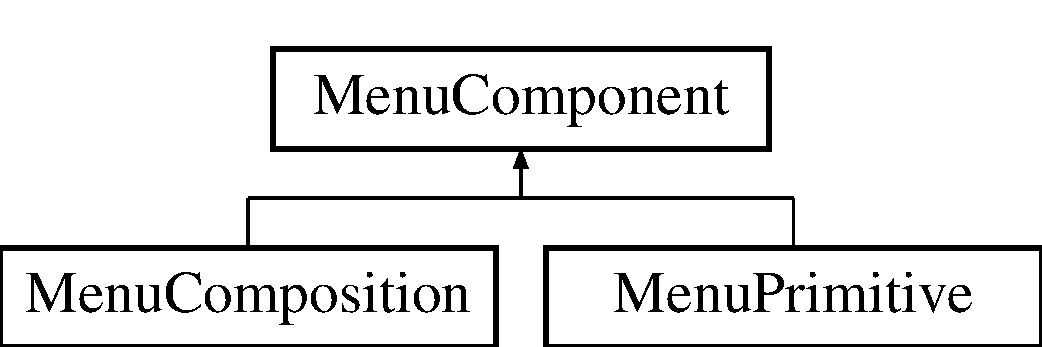
\includegraphics[height=2.000000cm]{classMenuComponent}
\end{center}
\end{figure}
\subsection*{Public Member Functions}
\begin{DoxyCompactItemize}
\item 
\hypertarget{classMenuComponent_a89f2473dbe9c3516ed67d6d4de941acd}{{\bfseries Menu\-Component} (string name, int hiearchy)}\label{classMenuComponent_a89f2473dbe9c3516ed67d6d4de941acd}

\item 
\hypertarget{classMenuComponent_aac643f9f5e0e1c146b76af7fa733396f}{virtual void {\bfseries Add} (\hyperlink{classMenuComponent}{Menu\-Component} $\ast$d)=0}\label{classMenuComponent_aac643f9f5e0e1c146b76af7fa733396f}

\item 
\hypertarget{classMenuComponent_abc5764fee211d1ce432fcd59584d2d32}{virtual void {\bfseries Remove} (\hyperlink{classMenuComponent}{Menu\-Component} $\ast$d)=0}\label{classMenuComponent_abc5764fee211d1ce432fcd59584d2d32}

\item 
\hypertarget{classMenuComponent_a65386099aca32e9b81b4eb973e60ece1}{virtual void {\bfseries Display} ()=0}\label{classMenuComponent_a65386099aca32e9b81b4eb973e60ece1}

\end{DoxyCompactItemize}
\subsection*{Protected Attributes}
\begin{DoxyCompactItemize}
\item 
\hypertarget{classMenuComponent_ac21370585d3f6a32f0b6ed8de00245b8}{string {\bfseries name\-\_\-}}\label{classMenuComponent_ac21370585d3f6a32f0b6ed8de00245b8}

\item 
\hypertarget{classMenuComponent_a391646eec6bf36ff63fecce621943b57}{int {\bfseries hiearchy\-\_\-}}\label{classMenuComponent_a391646eec6bf36ff63fecce621943b57}

\end{DoxyCompactItemize}


The documentation for this class was generated from the following files\-:\begin{DoxyCompactItemize}
\item 
Menu\-Component.\-h\item 
Menu\-Component.\-cpp\end{DoxyCompactItemize}

\hypertarget{classMenuComposition}{\section{Menu\-Composition Class Reference}
\label{classMenuComposition}\index{Menu\-Composition@{Menu\-Composition}}
}
Inheritance diagram for Menu\-Composition\-:\begin{figure}[H]
\begin{center}
\leavevmode
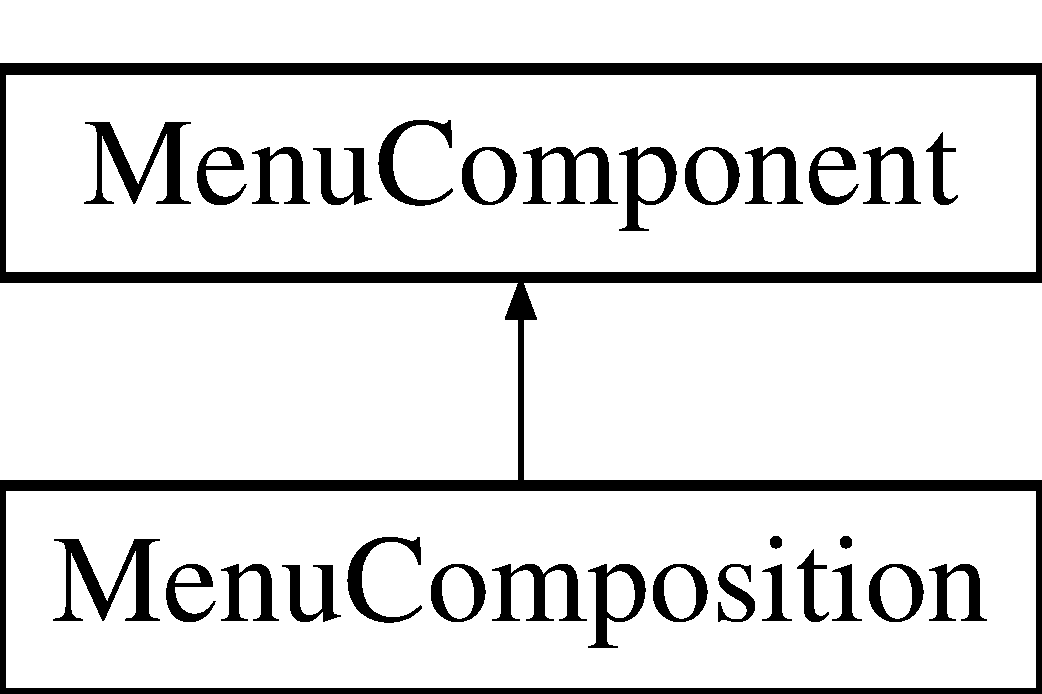
\includegraphics[height=2.000000cm]{classMenuComposition}
\end{center}
\end{figure}
\subsection*{Public Member Functions}
\begin{DoxyCompactItemize}
\item 
\hypertarget{classMenuComposition_aa8b77abb0d25ed9827bccca6e10bc396}{{\bfseries Menu\-Composition} (string name, int hierarchy)}\label{classMenuComposition_aa8b77abb0d25ed9827bccca6e10bc396}

\item 
\hypertarget{classMenuComposition_adc8165554a65bac3e2386895c5a6dfac}{void {\bfseries Add} (\hyperlink{classMenuComponent}{Menu\-Component} $\ast$d)}\label{classMenuComposition_adc8165554a65bac3e2386895c5a6dfac}

\item 
\hypertarget{classMenuComposition_a83f4e293743f306e960c3c1cf0b920ce}{void {\bfseries Remove} (\hyperlink{classMenuComponent}{Menu\-Component} $\ast$d)}\label{classMenuComposition_a83f4e293743f306e960c3c1cf0b920ce}

\item 
\hypertarget{classMenuComposition_a5f94b452c1a15c43e744ad72e1fb3895}{void {\bfseries Display} ()}\label{classMenuComposition_a5f94b452c1a15c43e744ad72e1fb3895}

\end{DoxyCompactItemize}
\subsection*{Additional Inherited Members}


The documentation for this class was generated from the following files\-:\begin{DoxyCompactItemize}
\item 
Menu\-Composition.\-h\item 
Menu\-Composition.\-cpp\end{DoxyCompactItemize}

\hypertarget{classMenuPrimitive}{\section{Menu\-Primitive Class Reference}
\label{classMenuPrimitive}\index{Menu\-Primitive@{Menu\-Primitive}}
}
Inheritance diagram for Menu\-Primitive\-:\begin{figure}[H]
\begin{center}
\leavevmode
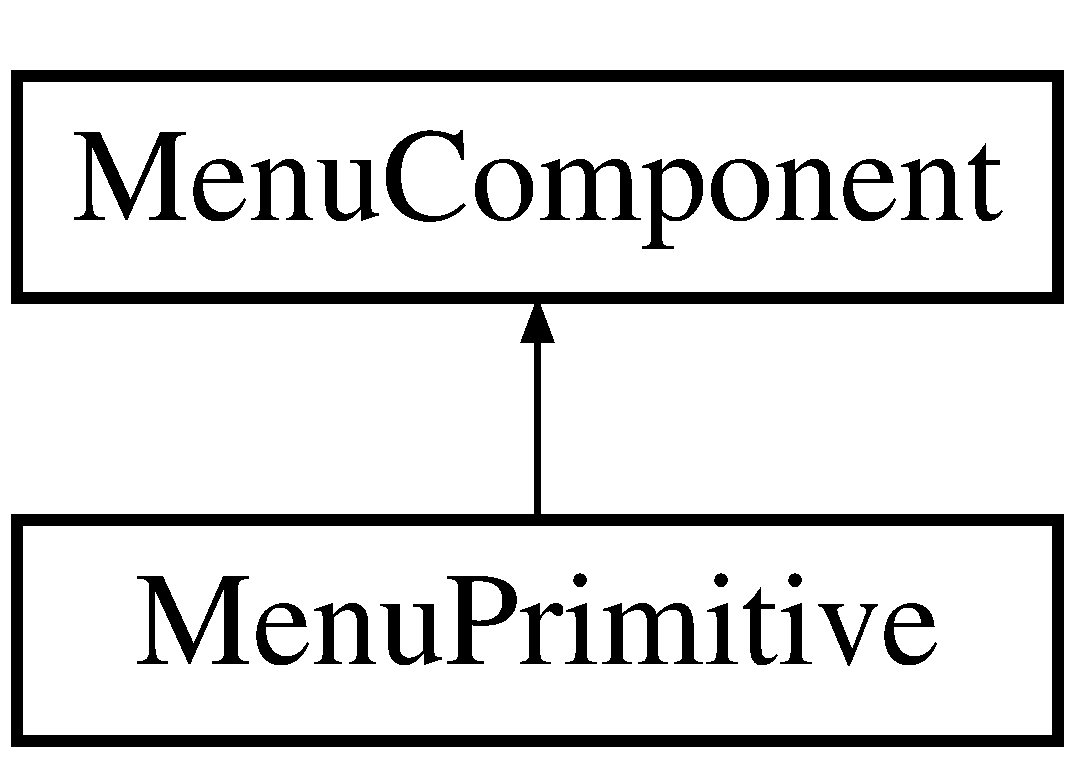
\includegraphics[height=2.000000cm]{dd/db3/classMenuPrimitive}
\end{center}
\end{figure}
\subsection*{Public Member Functions}
\begin{DoxyCompactItemize}
\item 
\hypertarget{classMenuPrimitive_a1676c1cd62bcee6034a7d393e422e4bd}{{\bfseries Menu\-Primitive} (string name, int hierarchy, int operation\-Num, string description, \hyperlink{classspi}{spi} $\ast$spi\-Dev)}\label{classMenuPrimitive_a1676c1cd62bcee6034a7d393e422e4bd}

\item 
\hypertarget{classMenuPrimitive_a452cdf28b74ebc7a2248ea044b457140}{void {\bfseries Add} (\hyperlink{classMenuComponent}{Menu\-Component} $\ast$d)}\label{classMenuPrimitive_a452cdf28b74ebc7a2248ea044b457140}

\item 
\hypertarget{classMenuPrimitive_a4c2032990cfc38456d65c7ad4213406d}{void {\bfseries Remove} (\hyperlink{classMenuComponent}{Menu\-Component} $\ast$d)}\label{classMenuPrimitive_a4c2032990cfc38456d65c7ad4213406d}

\item 
\hypertarget{classMenuPrimitive_acf5b9c7eff88942899b53459a2b45837}{void {\bfseries Display} ()}\label{classMenuPrimitive_acf5b9c7eff88942899b53459a2b45837}

\end{DoxyCompactItemize}
\subsection*{Additional Inherited Members}


The documentation for this class was generated from the following files\-:\begin{DoxyCompactItemize}
\item 
Menu\-Primitive.\-h\item 
Menu\-Primitive.\-cpp\end{DoxyCompactItemize}

\hypertarget{classmyDaemon}{\section{my\-Daemon Class Reference}
\label{classmyDaemon}\index{my\-Daemon@{my\-Daemon}}
}
\subsection*{Public Member Functions}
\begin{DoxyCompactItemize}
\item 
\hypertarget{classmyDaemon_a0e7924e217104938e0b4dd9e089a0c7d}{{\bfseries my\-Daemon} (const char $\ast$rundir, const char $\ast$pidfile\-Name)}\label{classmyDaemon_a0e7924e217104938e0b4dd9e089a0c7d}

\item 
\hypertarget{classmyDaemon_ad684d593d9d7ffcb7581faa965aa38f1}{int {\bfseries get\-Pid\-No} ()}\label{classmyDaemon_ad684d593d9d7ffcb7581faa965aa38f1}

\item 
\hypertarget{classmyDaemon_a0f1d30f6ada5fa68611ec491071c31dd}{void {\bfseries daemonize} ()}\label{classmyDaemon_a0f1d30f6ada5fa68611ec491071c31dd}

\end{DoxyCompactItemize}


The documentation for this class was generated from the following files\-:\begin{DoxyCompactItemize}
\item 
daemonize.\-h\item 
daemonize.\-cpp\end{DoxyCompactItemize}

\hypertarget{structserverParams}{\section{server\-Params Struct Reference}
\label{structserverParams}\index{server\-Params@{server\-Params}}
}
\subsection*{Public Attributes}
\begin{DoxyCompactItemize}
\item 
\hypertarget{structserverParams_a9acca3960089e8feda7c75f692f33350}{std\-::string {\bfseries \-\_\-servername} = \char`\"{}\char`\"{}}\label{structserverParams_a9acca3960089e8feda7c75f692f33350}

\item 
\hypertarget{structserverParams_ad2dd4bd8923b6843674c68d410c82a65}{std\-::string {\bfseries \-\_\-port\-No} = \char`\"{}\char`\"{}}\label{structserverParams_ad2dd4bd8923b6843674c68d410c82a65}

\end{DoxyCompactItemize}


The documentation for this struct was generated from the following file\-:\begin{DoxyCompactItemize}
\item 
Config\-File.\-h\end{DoxyCompactItemize}

\hypertarget{classspi}{\section{spi Class Reference}
\label{classspi}\index{spi@{spi}}
}


{\ttfamily \#include $<$spi.\-h$>$}

\subsection*{Public Member Functions}
\begin{DoxyCompactItemize}
\item 
virtual \hyperlink{classspi_aa7039ccea879c1194360b401427f7b93}{$\sim$spi} ()
\item 
\hypertarget{classspi_a34b00f5bd260681619fee418239048a0}{virtual void {\bfseries Serial\-Port\-Init} ()}\label{classspi_a34b00f5bd260681619fee418239048a0}

\item 
\hypertarget{classspi_a94309b811b02a030d1a37eca9e27b286}{virtual void {\bfseries Read\-Values} ()}\label{classspi_a94309b811b02a030d1a37eca9e27b286}

\item 
\hypertarget{classspi_ab4c9b1d0f205e9dfac00107bc8fe1729}{virtual void {\bfseries Run} ()}\label{classspi_ab4c9b1d0f205e9dfac00107bc8fe1729}

\item 
\hypertarget{classspi_a1676554345a6127503f10d117f5b242d}{virtual bool {\bfseries Calibrate} (int cal\-Type)}\label{classspi_a1676554345a6127503f10d117f5b242d}

\item 
\hypertarget{classspi_ab5338399676761d03e503fa8f55ff4f6}{int {\bfseries open\-Device} (const char $\ast$p\-Device)}\label{classspi_ab5338399676761d03e503fa8f55ff4f6}

\item 
\hypertarget{classspi_af0e4702c999e07c9d2655cae8d12d1a4}{void {\bfseries set\-Spi\-Speed} (uint32\-\_\-t spi\-Speed)}\label{classspi_af0e4702c999e07c9d2655cae8d12d1a4}

\item 
\hypertarget{classspi_a24d0af0b21a8f58127d18c7cf77f0fd2}{void {\bfseries set\-Spi\-Delay} (uint16\-\_\-t spi\-Delay)}\label{classspi_a24d0af0b21a8f58127d18c7cf77f0fd2}

\item 
\hypertarget{classspi_aa81694fe53868e64ad9ef35e9003ac96}{void {\bfseries set\-Bit\-Order} (uint8\-\_\-t bit\-Order)}\label{classspi_aa81694fe53868e64ad9ef35e9003ac96}

\item 
\hypertarget{classspi_aa1251c2275e3a868291c85106de2f44b}{void {\bfseries set\-Log} (System\-Log $\ast$pspi\-Sys\-Log)}\label{classspi_aa1251c2275e3a868291c85106de2f44b}

\item 
\hypertarget{classspi_a868d26f2805f7a0a5ab2b45fef847a3d}{void {\bfseries set\-Logger} (Logger $\ast$my\-Logger)}\label{classspi_a868d26f2805f7a0a5ab2b45fef847a3d}

\item 
virtual void \hyperlink{classspi_af6b5a441ef9014df209fa3803d0fa68f}{spi\-Init} ()
\end{DoxyCompactItemize}
\subsection*{Protected Member Functions}
\begin{DoxyCompactItemize}
\item 
\hypertarget{classspi_a01ec3f79a14b29cee3fed591c477ecc4}{virtual void {\bfseries Write\-Register} ()}\label{classspi_a01ec3f79a14b29cee3fed591c477ecc4}

\item 
\hypertarget{classspi_ab82db7e47c0788f8593c0213688043cd}{virtual int {\bfseries Read\-Register} ()}\label{classspi_ab82db7e47c0788f8593c0213688043cd}

\item 
int \hyperlink{classspi_ace5d4b909ab9a103ae676df30db26836}{spi\-Send\-Receive} (uint8\-\_\-t $\ast$p\-Tx\-Buf, int i\-Tx\-Len, uint8\-\_\-t $\ast$p\-Rx\-Buf, int i\-Rx\-Len)
\item 
void \hyperlink{classspi_ab1569afd18aaa3ecaacc5252dab1177c}{spi\-Init\-Bit\-Order} ()
\item 
\hypertarget{classspi_a911578bfdd06fb5a4572069213072e53}{void {\bfseries set\-Spi\-Wr\-Mode} (uint8\-\_\-t spi\-Wr\-Mode)}\label{classspi_a911578bfdd06fb5a4572069213072e53}

\item 
\hypertarget{classspi_aea783dd071bb43a6cd05bc9cf4acb0d4}{void {\bfseries set\-Spi\-Rd\-Mode} (uint8\-\_\-t spi\-Rd\-Mode)}\label{classspi_aea783dd071bb43a6cd05bc9cf4acb0d4}

\item 
\hypertarget{classspi_aeb466902f0246e674230656c36260417}{void {\bfseries set\-Spi\-Mode} (uint8\-\_\-t spi\-Mode)}\label{classspi_aeb466902f0246e674230656c36260417}

\item 
\hypertarget{classspi_a0ca79e4dfeb0520519aae82576881229}{void {\bfseries set\-Spi\-B\-P\-W} (uint8\-\_\-t spi\-B\-P\-W)}\label{classspi_a0ca79e4dfeb0520519aae82576881229}

\item 
\hypertarget{classspi_a00c5efd63b774a1d50d3e69c8a49e0fa}{void {\bfseries set\-Spi\-Max\-Speed} (uint32\-\_\-t max\-Speed)}\label{classspi_a00c5efd63b774a1d50d3e69c8a49e0fa}

\item 
void \hyperlink{classspi_a71d243d92efaea106a3ee14970ea5ebe}{current\-Time\-Date} ()
\end{DoxyCompactItemize}
\subsection*{Protected Attributes}
\begin{DoxyCompactItemize}
\item 
\hypertarget{classspi_a30e62f162a7381cb154ceba749c3f9ba}{System\-Log $\ast$ {\bfseries m\-\_\-my\-S\-P\-I\-Sys\-Log}}\label{classspi_a30e62f162a7381cb154ceba749c3f9ba}

\item 
\hypertarget{classspi_a6b36076244edf6f661198f69c6b89b2d}{Logger $\ast$ {\bfseries m\-\_\-p\-My\-Logger}}\label{classspi_a6b36076244edf6f661198f69c6b89b2d}

\item 
\hypertarget{classspi_aa584b9b3ec842ac93204341966469d4c}{std\-::string {\bfseries m\-\_\-date\-Time}}\label{classspi_aa584b9b3ec842ac93204341966469d4c}

\end{DoxyCompactItemize}


\subsection{Detailed Description}
S\-P\-I is a abstract base class that defines the functionality of S\-P\-I. the clas is an S\-P\-I and has a Sys log member to write messages ang error to the linux sys log utility. 

\subsection{Constructor \& Destructor Documentation}
\hypertarget{classspi_aa7039ccea879c1194360b401427f7b93}{\index{spi@{spi}!$\sim$spi@{$\sim$spi}}
\index{$\sim$spi@{$\sim$spi}!spi@{spi}}
\subsubsection[{$\sim$spi}]{\setlength{\rightskip}{0pt plus 5cm}spi\-::$\sim$spi (
\begin{DoxyParamCaption}
{}
\end{DoxyParamCaption}
)\hspace{0.3cm}{\ttfamily [virtual]}}}\label{classspi_aa7039ccea879c1194360b401427f7b93}
Virtual destructor 

\subsection{Member Function Documentation}
\hypertarget{classspi_a71d243d92efaea106a3ee14970ea5ebe}{\index{spi@{spi}!current\-Time\-Date@{current\-Time\-Date}}
\index{current\-Time\-Date@{current\-Time\-Date}!spi@{spi}}
\subsubsection[{current\-Time\-Date}]{\setlength{\rightskip}{0pt plus 5cm}void spi\-::current\-Time\-Date (
\begin{DoxyParamCaption}
{}
\end{DoxyParamCaption}
)\hspace{0.3cm}{\ttfamily [protected]}}}\label{classspi_a71d243d92efaea106a3ee14970ea5ebe}
void Current\-Time\-Date() Works out the current date and time when sensor data was read. \hypertarget{classspi_af6b5a441ef9014df209fa3803d0fa68f}{\index{spi@{spi}!spi\-Init@{spi\-Init}}
\index{spi\-Init@{spi\-Init}!spi@{spi}}
\subsubsection[{spi\-Init}]{\setlength{\rightskip}{0pt plus 5cm}void spi\-::spi\-Init (
\begin{DoxyParamCaption}
{}
\end{DoxyParamCaption}
)\hspace{0.3cm}{\ttfamily [virtual]}}}\label{classspi_af6b5a441ef9014df209fa3803d0fa68f}
Initializes the spi driver \hypertarget{classspi_ab1569afd18aaa3ecaacc5252dab1177c}{\index{spi@{spi}!spi\-Init\-Bit\-Order@{spi\-Init\-Bit\-Order}}
\index{spi\-Init\-Bit\-Order@{spi\-Init\-Bit\-Order}!spi@{spi}}
\subsubsection[{spi\-Init\-Bit\-Order}]{\setlength{\rightskip}{0pt plus 5cm}void spi\-::spi\-Init\-Bit\-Order (
\begin{DoxyParamCaption}
{}
\end{DoxyParamCaption}
)\hspace{0.3cm}{\ttfamily [protected]}}}\label{classspi_ab1569afd18aaa3ecaacc5252dab1177c}
Sets bit order \hypertarget{classspi_ace5d4b909ab9a103ae676df30db26836}{\index{spi@{spi}!spi\-Send\-Receive@{spi\-Send\-Receive}}
\index{spi\-Send\-Receive@{spi\-Send\-Receive}!spi@{spi}}
\subsubsection[{spi\-Send\-Receive}]{\setlength{\rightskip}{0pt plus 5cm}int spi\-::spi\-Send\-Receive (
\begin{DoxyParamCaption}
\item[{uint8\-\_\-t $\ast$}]{p\-Tx\-Buf, }
\item[{int}]{i\-Tx\-Len, }
\item[{uint8\-\_\-t $\ast$}]{p\-Rx\-Buf, }
\item[{int}]{i\-Rx\-Len}
\end{DoxyParamCaption}
)\hspace{0.3cm}{\ttfamily [protected]}}}\label{classspi_ace5d4b909ab9a103ae676df30db26836}
spi\-Send\-Receive has two functionalities sends$\vert$/writes to the S\-P\-I and send/receive from the S\-P\-I. The method make use of the linux function ioctl that performs the generic I/\-O operations. 

The documentation for this class was generated from the following files\-:\begin{DoxyCompactItemize}
\item 
spi.\-h\item 
spi.\-cpp\end{DoxyCompactItemize}

\hypertarget{structspiParams}{\section{spi\-Params Struct Reference}
\label{structspiParams}\index{spi\-Params@{spi\-Params}}
}
\subsection*{Public Attributes}
\begin{DoxyCompactItemize}
\item 
\hypertarget{structspiParams_a943b444e77f506b67c26334326be4caf}{uint8\-\_\-t {\bfseries bit\-Order}}\label{structspiParams_a943b444e77f506b67c26334326be4caf}

\item 
\hypertarget{structspiParams_abf2bae4035ced0c45ced2618c2150d66}{uint8\-\_\-t {\bfseries spi\-Wr\-Mode}}\label{structspiParams_abf2bae4035ced0c45ced2618c2150d66}

\item 
\hypertarget{structspiParams_a24ce28ae11d13edb3cc2611790f74448}{uint8\-\_\-t {\bfseries spi\-Rd\-Mode}}\label{structspiParams_a24ce28ae11d13edb3cc2611790f74448}

\item 
\hypertarget{structspiParams_adfa9ae8f40748929cd125f2a2627a490}{uint8\-\_\-t {\bfseries spi\-B\-P\-W}}\label{structspiParams_adfa9ae8f40748929cd125f2a2627a490}

\item 
\hypertarget{structspiParams_a29a2a33adc949277f980d55c573bcb07}{uint32\-\_\-t {\bfseries spi\-Speed}}\label{structspiParams_a29a2a33adc949277f980d55c573bcb07}

\item 
\hypertarget{structspiParams_ac6af66e49fb2c4f84b4fd09e7f2df147}{uint32\-\_\-t {\bfseries spi\-Max\-Speed}}\label{structspiParams_ac6af66e49fb2c4f84b4fd09e7f2df147}

\item 
\hypertarget{structspiParams_a7d276b4bdd88c78495a6d87919ea9664}{uint16\-\_\-t {\bfseries spi\-Delay}}\label{structspiParams_a7d276b4bdd88c78495a6d87919ea9664}

\item 
\hypertarget{structspiParams_a75dcaec546d7e6c605f854871b6cf2ca}{int {\bfseries fd}}\label{structspiParams_a75dcaec546d7e6c605f854871b6cf2ca}

\end{DoxyCompactItemize}
\subsection*{Static Public Attributes}
\begin{DoxyCompactItemize}
\item 
\hypertarget{structspiParams_a6f2ed69ae1dc110d7cd3de5e6b145a94}{static const char $\ast$ {\bfseries device}}\label{structspiParams_a6f2ed69ae1dc110d7cd3de5e6b145a94}

\end{DoxyCompactItemize}


The documentation for this struct was generated from the following file\-:\begin{DoxyCompactItemize}
\item 
spi.\-h\end{DoxyCompactItemize}

\hypertarget{structspiParamsStr}{\section{spi\-Params\-Str Struct Reference}
\label{structspiParamsStr}\index{spi\-Params\-Str@{spi\-Params\-Str}}
}
\subsection*{Public Attributes}
\begin{DoxyCompactItemize}
\item 
\hypertarget{structspiParamsStr_a9032047f10cab29967465daf89a0e6c5}{std\-::string {\bfseries \-\_\-device} = \char`\"{}\char`\"{}}\label{structspiParamsStr_a9032047f10cab29967465daf89a0e6c5}

\item 
\hypertarget{structspiParamsStr_a2d7123c02c09f548d9df499dde79c7e1}{std\-::string {\bfseries \-\_\-spi\-Mode} = \char`\"{}\char`\"{}}\label{structspiParamsStr_a2d7123c02c09f548d9df499dde79c7e1}

\item 
\hypertarget{structspiParamsStr_a91a52ca6f255d0f450c104f73b7e94a9}{std\-::string {\bfseries \-\_\-spi\-B\-P\-W} = \char`\"{}\char`\"{}}\label{structspiParamsStr_a91a52ca6f255d0f450c104f73b7e94a9}

\item 
\hypertarget{structspiParamsStr_ad69d2f6544326c2bd3ea9130fb11baec}{std\-::string {\bfseries \-\_\-spi\-Speed} = \char`\"{}\char`\"{}}\label{structspiParamsStr_ad69d2f6544326c2bd3ea9130fb11baec}

\item 
\hypertarget{structspiParamsStr_a50192a5701a61ca8a1c8fc26d450e27b}{std\-::string {\bfseries \-\_\-spi\-Delay} = \char`\"{}\char`\"{}}\label{structspiParamsStr_a50192a5701a61ca8a1c8fc26d450e27b}

\end{DoxyCompactItemize}


The documentation for this struct was generated from the following file\-:\begin{DoxyCompactItemize}
\item 
Config\-File.\-h\end{DoxyCompactItemize}

\hypertarget{structtimeDate}{\section{time\-Date Struct Reference}
\label{structtimeDate}\index{time\-Date@{time\-Date}}
}
\subsection*{Public Attributes}
\begin{DoxyCompactItemize}
\item 
\hypertarget{structtimeDate_a4513a3b33d516596a3270a42889d1d77}{std\-::time\-\_\-t {\bfseries time}}\label{structtimeDate_a4513a3b33d516596a3270a42889d1d77}

\item 
\hypertarget{structtimeDate_aba1a6fdf27de686648a1576d29833a9a}{std\-::string {\bfseries date}}\label{structtimeDate_aba1a6fdf27de686648a1576d29833a9a}

\end{DoxyCompactItemize}


The documentation for this struct was generated from the following file\-:\begin{DoxyCompactItemize}
\item 
spi.\-h\end{DoxyCompactItemize}

%--- End generated contents ---

% Index
\newpage
\phantomsection
\addcontentsline{toc}{chapter}{Index}
\printindex

\end{document}
